% This file was created with tikzplotlib v0.10.1.
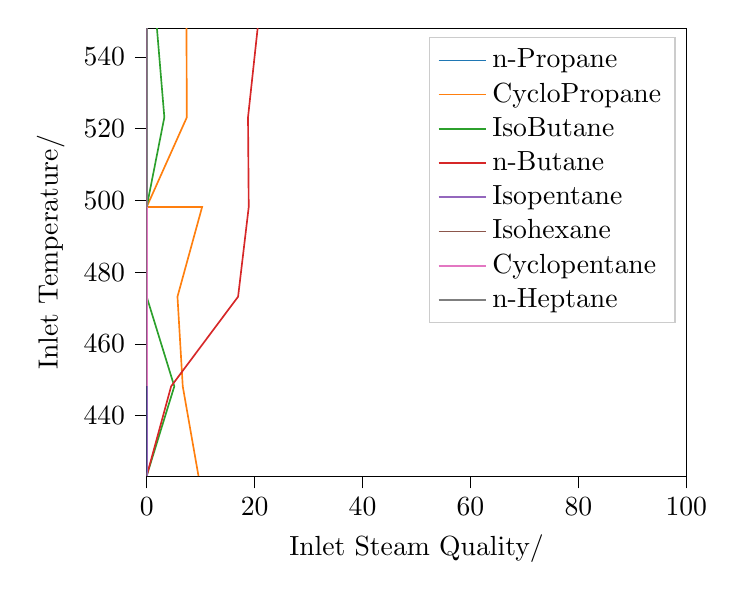
\begin{tikzpicture}

\definecolor{crimson2143940}{RGB}{214,39,40}
\definecolor{darkgray176}{RGB}{176,176,176}
\definecolor{darkorange25512714}{RGB}{255,127,14}
\definecolor{forestgreen4416044}{RGB}{44,160,44}
\definecolor{gray127}{RGB}{127,127,127}
\definecolor{lightgray204}{RGB}{204,204,204}
\definecolor{mediumpurple148103189}{RGB}{148,103,189}
\definecolor{orchid227119194}{RGB}{227,119,194}
\definecolor{sienna1408675}{RGB}{140,86,75}
\definecolor{steelblue31119180}{RGB}{31,119,180}

\begin{axis}[
legend cell align={left},
legend style={fill opacity=0.8, draw opacity=1, text opacity=1, draw=lightgray204},
tick align=outside,
tick pos=left,
x grid style={darkgray176},
xlabel={Inlet Steam Quality/\unit{\percent}},
xmin=0, xmax=100,
xtick style={color=black},
y grid style={darkgray176},
ylabel={Inlet Temperature/\unit{\K}},
ymin=423, ymax=548,
ytick style={color=black}
]
\addplot [semithick, steelblue31119180]
table {%
0 548.15
0 523.15
0 498.15
0 473.15
0 448.15
0 423.15
};
\addlegendentry{n-Propane}
\addplot [semithick, darkorange25512714]
table {%
7.37459290074186 548.15
7.44024453282398 523.15
0 498.15
10.2728103470557 498.15
5.70867385369574 473.15
6.68611121421122 448.15
9.60181428355033 423.15
};
\addlegendentry{CycloPropane}
\addplot [semithick, forestgreen4416044]
table {%
1.89072290870401 548.15
3.27471307641813 523.15
0 498.15
0 473.15
5.12368290885298 448.15
0 423.15
};
\addlegendentry{IsoButane}
\addplot [semithick, crimson2143940]
table {%
20.5758201963607 548.15
18.7789988175102 523.15
18.9121530717588 498.15
16.939788265825 473.15
4.53004342488796 448.15
0 423.15
};
\addlegendentry{n-Butane}
\addplot [semithick, mediumpurple148103189]
table {%
0 548.15
0 523.15
0 498.15
0 473.15
0 448.15
0 423.15
};
\addlegendentry{Isopentane}
\addplot [semithick, sienna1408675]
table {%
0 548.15
0 523.15
0 498.15
0 473.15
0 448.15
};
\addlegendentry{Isohexane}
\addplot [semithick, orchid227119194]
table {%
0 548.15
0 523.15
0 498.15
0 473.15
0 448.15
};
\addlegendentry{Cyclopentane}
\addplot [semithick, gray127]
table {%
0 548.15
0 523.15
0 498.15
};
\addlegendentry{n-Heptane}
\end{axis}

\end{tikzpicture}
